\documentclass{beamer}
\usetheme{CambridgeUS}
\usepackage[french]{babel}
\usepackage{fontspec}
\usepackage{graphicx}
\usepackage{textcomp}
\usepackage{import}
\usepackage{tabu}
\usepackage{colortbl}
\usepackage{arydshln}
\usepackage{multirow}
\usepackage{pgffor}

%\usepackage{minted}
%\usemintedstyle{trac}

% More vertical spacing in tabu lines
\tabulinesep=1.5mm

\graphicspath{{figures/}}
\useinnertheme{rectangles}
\setbeamertemplate{blocks}[default]

\title[Environnement pour l'exploration visuelle]{Environnement logiciel pour l'apprentissage de l'exploration visuelle d'une image}
\author{Louis Cuni \and Pablo Donato}
\institute[]{Université Pierre et Marie Curie -- Paris VI}
\date{2 mai 2017}
\subject{Projet de recherche}

\setcounter{tocdepth}{1}
\AtBeginSection[]
{
    \begin{frame}
        \frametitle{Sommaire}
        \tableofcontents[currentsection]
    \end{frame}
}


%\begin{frame}
    %\frametitle{Titre}
    %\begin{columns}[T]
        %\begin{column}{.48\textwidth}
            %\center
            %\begin{block}{Bloc 1}
                %\begin{itemize}
                    %\item Item 1
                    %\item Item 2
                    %\item Item 3
                %\end{itemize}
            %\end{block}
        %\end{column}
        %\begin{column}{.48\textwidth}
            %\begin{figure}
                %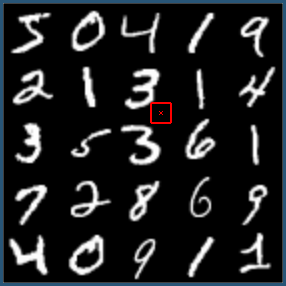
\includegraphics[height=0.5\textheight]{numgrid.png}
            %\end{figure}
        %\end{column}
    %\end{columns}
%\end{frame}


\begin{document}

\frame{\titlepage}

\section{Introduction}

\begin{frame}
    \frametitle{Contexte}
    \begin{columns}[T]
        \begin{column}{.48\textwidth}
            \center
            \begin{block}{Environnement}
                TODO
            \end{block}
            \begin{block}{Agent}
                TODO
            \end{block}
        \end{column}
        \begin{column}{.48\textwidth}
            \begin{figure}
                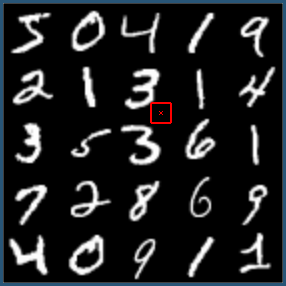
\includegraphics[height=0.5\textheight]{numgrid.png}
            \end{figure}
        \end{column}
    \end{columns}
\end{frame}

\begin{frame}
    \frametitle{Interaction agent-environnement}
    \center
    \begin{figure}
        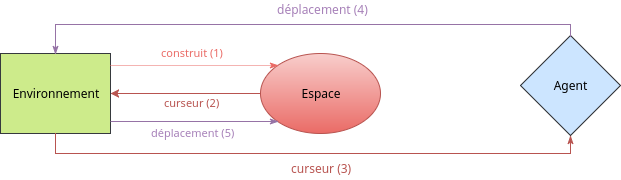
\includegraphics[width=0.9\textwidth]{agent_env_loop.png}
    \end{figure}
    \vspace{3em}
    \begin{enumerate}
        \item Construction de l'\textbf{espace}
        \item Boucle d'interaction
    \end{enumerate}
\end{frame}

\section{Environnement}

\section{Agent}

\begin{frame}
    \frametitle{Réseaux de neurones}
    \begin{columns}[T]
        \begin{column}{.48\textwidth}
            \begin{figure}
                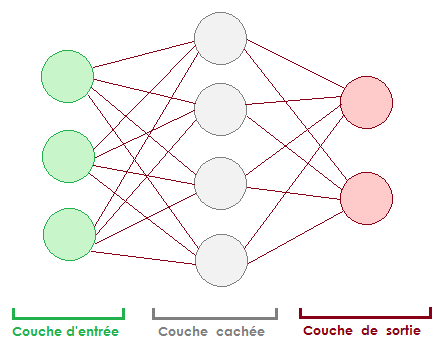
\includegraphics[width=\textwidth]{neuralnet.png}
            \end{figure}
        \end{column}
        \begin{column}{.48\textwidth}
            \begin{figure}
                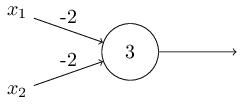
\includegraphics[width=0.8\textwidth]{neuron.png}
            \end{figure}
            \begin{block}{}
                \center
                Commentaires ?
            \end{block}
        \end{column}
    \end{columns}
\end{frame}

\begin{frame}
    \frametitle{Prédicteurs}
    \begin{figure}
        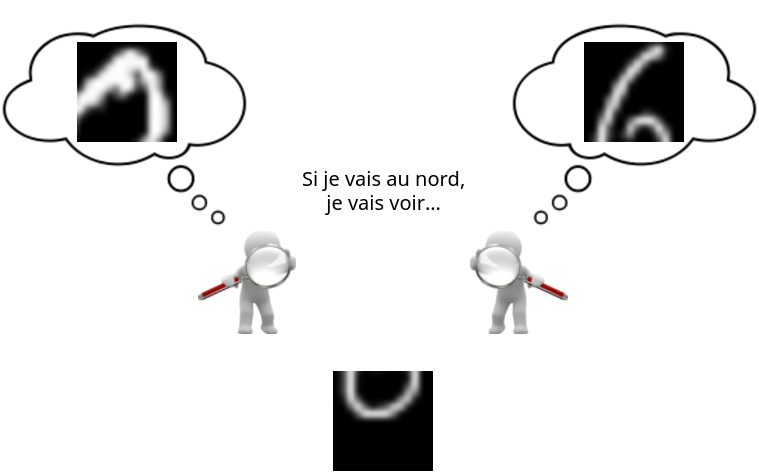
\includegraphics[width=0.9\textwidth]{slide_predicter.png}
    \end{figure}
\end{frame}

\newcommand{\predicterguy}[1]{
    \begin{minipage}{.15\textwidth}
        \center
        \includegraphics[width=0.75\linewidth]{predicter_guy_#1.png}
    \end{minipage}}
\newcommand{\pls}{\cellcolor{blue!20}}
\newcommand{\win}{\cellcolor{green!20}}
\begin{frame}
    \frametitle{Prise de décisions}
    \fontsize{7pt}{7}\selectfont
    \center
    \begin{tabu}{|c|c|c|c|} \hline
        \predicterguy{1} & \predicterguy{2} & \predicterguy{3} & $t$ \\ \hline
        0 & 0 & 0 & \multirow{2}{*}{0} \\ \cdashline{1-3}[1pt/1.5pt]
        0 & 0 & 0 & \\ \hline
        0.81 & 0.86 \pls & 0.83 & \multirow{2}{*}{1} \\ \cdashline{1-3}[1pt/1.5pt]
        0 & 1 & 0 & \\ \hline
        0.84 \pls & 0.83 & 0.80 & \multirow{2}{*}{2} \\ \cdashline{1-3}[1pt/1.5pt]
        1 & 1 & 0 & \\ \hline
        0.82 & 0.89 \pls & 0.85 & \multirow{2}{*}{3} \\ \cdashline{1-3}[1pt/1.5pt]
        1 & 2 & 0 & \\ \hline
        0.83 & 0.91 \win & 0.86 & \multirow{2}{*}{4} \\ \cdashline{1-3}[1pt/1.5pt]
        1 & 3 & 0 & \\ \hline
    \end{tabu}
\end{frame}

\begin{frame}
    \frametitle{Exemple d'une séquence d'identification}
    \center
    \foreach \n in {0,...,11}{
        \only<\n>{
        \begin{figure}
            \includegraphics[height=0.75\textheight]{ident_seq/ident_seq_\n.png}
        \end{figure}}}
\end{frame}

\section{Étude expérimentale}

\section{Conclusion}

\end{document}
